\begin{figure}[h]
  \centering
  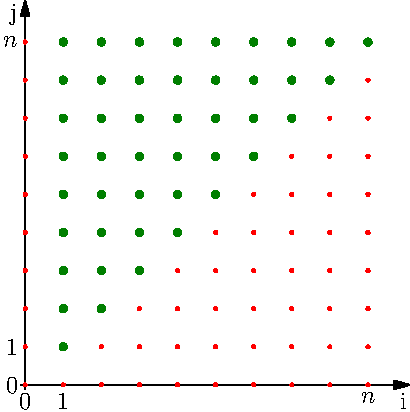
\includegraphics{./Csomm4_1.pdf}
  % Csomm4_1.pdf: 0x0 pixel, 0dpi, 0.00x0.00 cm, bb=
  \caption{Domaine de sommation triangulaire}
  \label{fig:Csomm4_1}
\end{figure}

\begin{enumerate}
  \item On montre que 
\begin{displaymath}
 S = \sum_{k=a}^b k = \underset{\text{moy des extrémités}}{\underbrace{\frac{1}{2}(a+b)}}
                   \underset{\text{nb de termes}}{\underbrace{(b-a+1)}}
\end{displaymath}
Cette formule s'obtient par exemple avec un changement d'indice de sommation
\begin{displaymath}
2S = \sum_{k=a}^b k + \sum_{k=a}^b (a+b-k) = \sum_{k=a}^b (a+b) = (b-a+1)(a+b)
\end{displaymath}

  \item 
\begin{enumerate}
  \item Le domaine de sommation est le triangle au dessus de la diagonale représenté en figure \ref{fig:Csomm4_1}. Noter que les indices commencent à $1$.
  \item Notons $S_2(n)$ la somme proposée et sommons d'abord sur les lignes.
\begin{displaymath}
S_2(n) = \sum_{j=1}^{n}\sum_{i=1}^{j}\frac{i}{j}
= \sum_{j=1}^{n}\left( \sum_{i=1}^{j}i\right)\frac{1}{j}
= \sum_{j=1}^{n}\frac{j(j+1)}{2j}
= \frac{1}{2}\sum_{k=2}^{n+1}k = \frac{n(n+3)}{4}
\end{displaymath}
\end{enumerate}

  \item Notons $S_3(n)$ la somme. Elle porte sur les triplets $(i,j,k)$ tels que $1\leq i \leq j \leq k \leq n$. On regroupe ces triplets suivant les valeurs du troisième indice.
\begin{multline*}
  S_3(n) = \sum_{k=1}^n\left( \sum_{i=1}^k \sum_{j=i}^k\frac{i}{jk}\right) 
= \sum_{k=1}^n\left( \sum_{i=1}^k \sum_{j=i}^k\frac{i}{j}\right)\frac{1}{k}
= \sum_{k=1}^n \frac{S_2(k)}{k}
= \sum_{k=1}^n \frac{k+3}{4} \\
=\frac{n(n+7)}{8}
\end{multline*}

  \item Notons $S_k(n)$ la somme que l'on nous demande de considérer. Cette notation est cohérente avec les premières questions. On raisonne par récurrence, les formules sont valides pour $k=2$ et $3$. Pour passer de $k-1$ à $k$, on regroupe encore les $k$-uplets suivant la valeur du dernier indice
\begin{multline*}
S_k(n) = \sum_{i_k=1}^{n}\left( \sum_{1\leq i_1 \leq i_2 \leq \cdots \leq i_{k-1}\leq i_{k}} \frac{i_1}{i_2 i_3 \cdots i_{k-1} i_k}\right) \\
= \sum_{i_k=1}^{n}\left( \sum_{1\leq i_1 \leq i_2 \leq \cdots \leq i_{k-1}\leq i_{k}} \frac{i_1}{i_2 i_3 \cdots i_{k-1}}\right)\frac{1}{i_k}
= \sum_{i_k=1}^{n} S_{k-1}(i_k)\frac{1}{i_k}\\
= \sum_{i_k=1}^{n}\frac{i_k(i_k+2^{k-1}-1)}{2^{k-1}i_k}
= \frac{1}{2^{k-1}}\frac{1}{2}n(2^{k-1}+2^{k-1}+n-1)
= \frac{n(2^{k}+n-1)}{2^{k}}
\end{multline*}
car on retrouve une somme de termes consécutifs entre $2^{k-1}$ et $2^{k-1}+n-1$.
\end{enumerate}
